\documentclass[12pt,a4paper]{article}
\usepackage[french]{babel}
\usepackage[utf8]{inputenc}
\usepackage[T1]{fontenc}
\usepackage{geometry}
\usepackage{xcolor}
\usepackage{graphicx}
\usepackage{enumitem}
\usepackage{tabularx}
\usepackage{booktabs}
\usepackage{amsmath}
\usepackage{fancyhdr}
\usepackage{hyperref}
\usepackage{mdframed}
\usepackage{longtable}

\geometry{margin=2.5cm}

\definecolor{primary}{RGB}{41, 128, 185}
\definecolor{secondary}{RGB}{52, 73, 94}
\definecolor{accent}{RGB}{231, 76, 60}
\definecolor{lightblue}{RGB}{235, 245, 251}
\definecolor{lightorange}{RGB}{253, 235, 208}
\definecolor{success}{RGB}{39, 174, 96}

\hypersetup{
    colorlinks=true,
    linkcolor=primary,
    urlcolor=primary
}

\pagestyle{fancy}
\fancyhf{}
\fancyhead[L]{\textbf{PEKEGNO} -- Guide du Modèle de Données}
\fancyhead[R]{\thepage}

\setlength{\parindent}{0pt}
\setlength{\parskip}{6pt}

\newmdenv[backgroundcolor=lightblue!40, linecolor=primary, roundcorner=5pt]{infobox}
\newmdenv[backgroundcolor=lightorange!40, linecolor=orange!60!black, roundcorner=5pt]{exemplebox}
\newmdenv[backgroundcolor=green!5, linecolor=success, roundcorner=5pt]{resume}

\begin{document}

\thispagestyle{empty}
\vspace*{2cm}
\begin{center}
    {\Huge \textbf{PEKEGNO}}\\[0.5cm]
    {\Large Guide du Modèle de Données}\\[1cm]
    \textcolor{primary}{\rule{\textwidth}{3pt}}\\[1cm]
    {\LARGE Phase 2 -- Cœur Métier}\\[0.3cm]
    {\Large Services, Formations, Formateurs et Inscriptions}\\[1.5cm]
    \vfill
    \begin{tabularx}{0.7\textwidth}{>{\raggedleft\arraybackslash}X >{\raggedright\arraybackslash}X}
        \textbf{Document} & Explication pas à pas \\
        \textbf{Niveau} & Débutant \\
        \textbf{Version} & 1.0 \\
    \end{tabularx}
\end{center}
\newpage

\tableofcontents
\newpage

% ===================================================================
\section{Pour commencer, c'est quoi tout ça ?}
% ===================================================================

Imagine que tu dois construire une bibliothèque. Avant de mettre les livres sur les étagères, il faut dessiner un plan :
\begin{itemize}
    \item \textbf{Combien d'étagères ?}
    \item \textbf{Quelle taille pour chaque étagère ?}
    \item \textbf{Comment sont rangés les livres ?}
\end{itemize}

Le \textbf{Modèle Conceptuel de Données (MCD)} et le \textbf{Modèle Logique de Données (MLD)}, c'est pareil, mais pour une application web. C'est le plan de construction de la base de données.

Dans ce guide, on va expliquer le modèle de la \textbf{Phase 2 de PEKEGNO}, c'est-à-dire la partie qui gère :
\begin{itemize}
    \item Les \textbf{services} et \textbf{formations} proposés
    \item Les \textbf{modules} de formation (vidéos, PDF)
    \item Les \textbf{formateurs} qui enseignent
    \item Les \textbf{inscriptions} des apprenants
    \item Les \textbf{paiements} et \textbf{échéances}
\end{itemize}

\bigskip

\begin{resume}
    \textbf{En une phrase :} Le MCD c'est le dessin en gros (les concepts), le MLD c'est le plan détaillé (les tables avec leurs colonnes).
\end{resume}


% ===================================================================
\section{Le MCD expliqué pas à pas}
% ===================================================================

Le MCD (Modèle Conceptuel de Données) répond à la question : \textbf{« De quoi parle-t-on ? »}. Il montre les grandes idées (les \textbf{entités}) et comment elles sont reliées entre elles (les \textbf{relations}).

\subsection{Les petites cartes (entités)}

Chaque encadré dans le diagramme représente une \textbf{entité}, c'est-à-dire une chose importante pour l'application. Par exemple :
\begin{itemize}
    \item \textbf{SERVICE} = un service ou une activité vendue par PEKEGNO
    \item \textbf{FORMATION} = une formation (un type particulier de service)
    \item \textbf{MODULE} = une leçon dans une formation
    \item \textbf{INSCRIPTION} = le fait qu'une personne s'inscrive à une formation
\end{itemize}

Dans un encadré, la partie du haut (après le \texttt{+}) contient les \textbf{identifiants} et la partie du bas contient les \textbf{propriétés}.

\subsection{Les traits entre les cartes (relations)}

Quand deux entités sont reliées par un trait, ça veut dire qu'elles ont un lien. Par exemple :
\begin{itemize}
    \item Une \textbf{FORMATION} est \textbf{composée de} plusieurs \textbf{MODULES}
    \item Un \textbf{SERVICE} peut avoir une \textbf{PROMOTION}
\end{itemize}

\subsection{Les nombres sur les traits (cardinalités)}

Les petits nombres comme \texttt{(1,1)} ou \texttt{(0,N)} qu'on voit sur chaque trait s'appellent des \textbf{cardinalités}. Ils disent \textbf{combien de fois} une entité peut être liée à l'autre.

\subsubsection{Comment lire une cardinalité ?}

Prenons l'exemple :

CATÉGORIE --- (1,N) --- (1,1) --- SERVICE


\begin{itemize}
    \item \texttt{(1,N)} à côté de CATÉGORIE : \textbf{Une catégorie peut classer 1, 2, 3... ou N services}. N veut dire \textbf{beaucoup} (on ne met pas de limite).
    \item \texttt{(1,1)} à côté de SERVICE : \textbf{Un service appartient à exactement 1 catégorie}. Pas 0, pas 2 : exactement 1.
\end{itemize}

\begin{exemplebox}
    \textbf{Exemple concret :} \\
    La catégorie \textit{« Bien-être »} peut contenir plusieurs services comme \textit{« Massage relaxant »}, \textit{« Soin du visage »}. \\
    Mais le service \textit{« Massage relaxant »} ne peut être que dans UNE seule catégorie : \textit{« Bien-être »}.
\end{exemplebox}

\subsubsection{Les différentes cardinalités}

\noindent\begin{tabularx}{\textwidth}{l X}
    \toprule
    \textbf{Symbole} & \textbf{Ça veut dire quoi ?} \\
    \midrule
    \texttt{(1,1)} & \textbf{Exactement un} -- obligatoire. On ne peut pas faire sans. \\
    \texttt{(0,1)} & \textbf{Zéro ou un} -- optionnel. On peut avoir ou ne pas avoir. \\
    \texttt{(1,N)} & \textbf{Au moins un, et possiblement plusieurs} -- obligatoire et multiple. \\
    \texttt{(0,N)} & \textbf{Zéro, un ou plusieurs} -- optionnel et multiple. \\
    \bottomrule
\end{tabularx}

\vspace{12pt}

\begin{infobox}
    \textbf{Petit moyen mnémotechnique :}
    \begin{itemize}
        \item \texttt{1} = \textbf{obligatoire} (tu DOIS en avoir un)
        \item \texttt{0} = \textbf{optionnel} (tu PEUX ne pas en avoir)
        \item \texttt{N} = \textbf{plusieurs} (tu PEUX en avoir beaucoup)
    \end{itemize}
\end{infobox}

% ===================================================================
\section{Les entités du MCD une par une}
% ===================================================================

\subsection{UTILISATEUR (vient de la Phase 1)}

\begin{minipage}[t]{0.65\textwidth}
C'est \textbf{une personne} qui utilise l'application. \\
\textbf{Propriétés :} id, nom, email, rôle.

\vspace{4pt}
\fcolorbox{primary}{lightblue!20}{\parbox{\textwidth}{\small
\textbf{Dans la vraie vie :} \\
Topo Boss (user) a le rôle \textit{Direction}. \\
Koffi (user) a le rôle \textit{Commercial}. \\
Amara (user) a le rôle \textit{Formateur}. \\
}} 
\end{minipage}

\vspace{12pt}

Un même utilisateur peut être \textbf{formateur} (enseigner des formations) ET \textbf{apprenant} (suivre des formations). C'est son rôle qui détermine ce qu'il a le droit de faire.

\subsection{SERVICE}

\noindent\begin{minipage}[t]{0.3\textwidth}
\fcolorbox{orange!60!black}{lightorange!20}{\parbox{\textwidth}{\small
\textbf{SERVICE} \\
-- nom \\
-- description \\
-- prix \\
-- couverture \\
-- vidéo
}}
\end{minipage}
\hfill
\begin{minipage}[t]{0.65\textwidth}
C'est \textbf{ce que PEKEGNO vend}. Par exemple : une consultation, une formation, un abonnement.

\vspace{4pt}
\fcolorbox{primary}{lightblue!20}{\parbox{\textwidth}{\small
\textbf{Exemple :} Service \textit{« Formation Excel »} avec prix 50 000 FCFA, décrite comme \textit{« Apprenez Excel en 2 semaines »}.
}} 
\end{minipage}

\subsection{PROMOTION}

Quand un service est \textbf{en promo}, on note dans cette entité : le prix réduit, la date de début et la date de fin. Une promotion est toujours liée à \textbf{un seul service}.

\begin{exemplebox}
    \textbf{Exemple :} Le service \textit{« Formation Excel »} a une promotion du 1er au 15 août à 35 000 FCFA au lieu de 50 000.
\end{exemplebox}

\subsection{HISTORIQUE\_PRIX}

Chaque fois qu'on change le prix d'un service, on l'enregistre ici. Cela permet de voir \textbf{l'historique des prix} dans le temps.

\subsection{FORMATION}

C'est un \textbf{type particulier de service}. Tous les services ne sont pas des formations, mais toutes les formations sont des services.

\begin{itemize}
    \item \textbf{FORMATION PRÉSENTIELLE} : on se déplace dans une salle. On peut payer en plusieurs fois (acompte + échéances).
    \item \textbf{FORMATION DISTANCIELLE} : on suit en ligne. Paiement obligatoire en ligne (Orange Money, MTN, etc.).
\end{itemize}

\noindent\fcolorbox{primary}{lightblue!20}{\parbox{\textwidth}{\small
\textbf{Exemple :} La formation \textit{« Excel »} est de type \textit{Présentiel}, dure 5 jours, coûte 50 000 FCFA avec un acompte de 15 000 FCFA et 2 échéances.
}}

\subsection{MODULE}

Une formation est \textbf{découpée en modules}. Chaque module est une leçon avec :
\begin{itemize}
    \item Un \textbf{nom} et un \textbf{ordre} (Module 1, Module 2, \ldots)
    \item Un \textbf{type} : \texttt{VIDEO} ou \texttt{PDF}
    \item Une \textbf{vidéo} (si type VIDEO) ou un \textbf{PDF} (si type PDF)
    \item Un \textbf{formateur} qui l'enseigne (c'est un UTILISATEUR avec le rôle \textit{Formateur})
\end{itemize}

\begin{exemplebox}
    \textbf{Exemple :} Formation \textit{« Excel »} a 3 modules : \\
    Module 1 -- \textit{« Les bases d'Excel »} (VIDEO, 30 min) \\
    Module 2 -- \textit{« Les formules »} (VIDEO, 45 min) \\
    Module 3 -- \textit{« Exercice pratique »} (PDF, à télécharger)
\end{exemplebox}

\subsection{INSCRIPTION}

Quand une personne s'inscrit à une formation, on crée une \textbf{inscription}. Elle contient :
\begin{itemize}
    \item Les \textbf{informations de la personne} (nom, prénom, téléphone, email, ville, pays, quartier, nationalité, occupation)
    \item Le \textbf{suivi financier} (montant total, montant payé, solde restant)
    \item Le \textbf{statut} (inscrit, en cours, terminé, annulé)
\end{itemize}

L'apprenant est relié à un \textbf{UTILISATEUR} (si son compte a déjà été créé).

\subsection{ECHEANCE}

Pour les formations présentielles payées en plusieurs fois, on crée des \textbf{échéances}. Chaque échéance a :
\begin{itemize}
    \item Un \textbf{montant} à payer
    \item Une \textbf{date d'échéance} (date limite)
    \item Un \textbf{statut} (impayé, payé, en retard)
    \item Une \textbf{pénalité} si l'échéance est dépassée
\end{itemize}

\subsection{PROGRESSION}

Pour chaque module d'une formation, on suit la \textbf{progression} de l'apprenant :
\begin{itemize}
    \item \texttt{pas\_commencé} → \texttt{en\_cours} → \texttt{terminé}
    \item Avec les dates de début et de fin
\end{itemize}

% ===================================================================
\section{Toutes les relations du MCD expliquées}
% ===================================================================

\subsection{CATÉGORIE -- SERVICE : « classifie »}


CATÉGORIE --- (1,N) --- (1,1) --- SERVICE


\begin{itemize}
    \item Une catégorie peut \textbf{classer plusieurs services} (N).
    \item Un service appartient à \textbf{exactement une catégorie} (1,1).
\end{itemize}

\begin{exemplebox}
    \small
    Catégorie \textit{« Informatique »} \(\rightarrow\) Service \textit{« Formation Excel »}, \textit{« Initiation Python »}, \textit{« maintenance PC »}\\
    Le service \textit{« Formation Excel »} \(\rightarrow\) seulement la catégorie \textit{« Informatique »}, pas \textit{« Bien-être »}.
\end{exemplebox}

\subsection{AGENCE -- SERVICE : « propose »}


AGENCE --- (1,N) --- (0,1) --- SERVICE


\begin{itemize}
    \item Une agence peut \textbf{proposer plusieurs services} (N).
    \item Un service peut être proposé par \textbf{0 ou 1 agence} (0,1). Parfois un service est rattaché directement à un département sans passer par une agence.
\end{itemize}

\subsection{DÉPARTEMENT -- SERVICE : « rattaché à »}


DÉPARTEMENT --- (1,N) --- (0,1) --- SERVICE


\begin{itemize}
    \item Un département peut avoir \textbf{plusieurs services} (N).
    \item Un service est rattaché à \textbf{0 ou 1 département} (0,1).
\end{itemize}

\subsection{SERVICE -- HISTORIQUE\_PRIX : « historique »}


SERVICE --- (1,1) --- (0,N) --- HISTORIQUE\_PRIX


\begin{itemize}
    \item Un service a \textbf{un historique de prix} (il peut avoir eu plusieurs prix dans le temps).
    \item Chaque entrée d'historique appartient à \textbf{exactement un service}.
\end{itemize}

\subsection{SERVICE -- PROMOTION : « promotion »}


SERVICE --- (1,1) --- (0,N) --- PROMOTION


\begin{itemize}
    \item Un service peut avoir \textbf{plusieurs promotions} (à différentes périodes).
    \item Chaque promotion concerne \textbf{exactement un service}.
\end{itemize}

\subsection{SERVICE -- FORMATION : « formation »}


SERVICE --- (0,1) --- (1,1) --- FORMATION


C'est la relation la plus importante à comprendre :

\begin{itemize}
    \item Une formation \textbf{est obligatoirement liée à un service} (1,1). Elle hérite du nom, du prix, de la description, etc.
    \item Un service peut \textbf{être ou ne pas être une formation} (0,1). Certains services ne sont pas des formations (ex: une consultation, un abonnement).
\end{itemize}

\begin{exemplebox}
    \small
    Le service \textit{« Formation Excel »} \(\rightarrow\) a une formation associée (type Présentiel, 5 jours).\\
    Le service \textit{« Massage relaxant »} \(\rightarrow\) n'a PAS de formation associée (c'est juste un service simple).
\end{exemplebox}

\subsection{FORMATION -- MODULE : « composé de »}


FORMATION --- (1,1) --- (0,N) --- MODULE


\begin{itemize}
    \item Une formation \textbf{est composée d'au moins un module} (elle peut en avoir plusieurs : 0,N).
    \item Chaque module appartient à \textbf{exactement une formation} (1,1).
\end{itemize}

\begin{exemplebox}
    \small
    Formation \textit{« Excel »} \(\rightarrow\) Module 1, Module 2, Module 3. \\
    Module 1 \(\rightarrow\) uniquement la formation \textit{« Excel »}, pas \textit{« Python »}.
\end{exemplebox}

\subsection{MODULE -- UTILISATEUR : « dispensé par »}


MODULE --- (0,N) --- (0,1) --- UTILISATEUR


\begin{itemize}
    \item Un module peut être \textbf{dispensé par 0 ou 1 formateur} (0,1). Parfois aucun formateur n'est encore attribué.
    \item Un utilisateur (avec le rôle \textit{Formateur}) peut \textbf{dispenser plusieurs modules} (N).
\end{itemize}

\subsection{FORMATION -- INSCRIPTION : « inscrit »}


FORMATION --- (1,1) --- (0,N) --- INSCRIPTION


\begin{itemize}
    \item Une formation peut \textbf{recevoir plusieurs inscriptions} (N).
    \item Chaque inscription concerne \textbf{exactement une formation} (1,1).
\end{itemize}

\subsection{UTILISATEUR -- INSCRIPTION : « s'inscrit à »}


UTILISATEUR --- (0,N) --- (1,1) --- INSCRIPTION


\begin{itemize}
    \item Un utilisateur (l'apprenant) peut avoir \textbf{plusieurs inscriptions} (dans différentes formations).
    \item Chaque inscription appartient à \textbf{exactement un utilisateur} (1,1).
\end{itemize}

\begin{exemplebox}
    \small
    L'utilisateur \textit{Jean} est inscrit à \textit{« Excel »} et à \textit{« Marketing »}. \\
    L'inscription \textit{« Jean → Excel »} n'appartient qu'à Jean, pas à Paul.
\end{exemplebox}

\subsection{INSCRIPTION -- ECHEANCE : « échelonné en »}


INSCRIPTION --- (1,1) --- (0,N) --- ECHEANCE


\begin{itemize}
    \item Une inscription peut être \textbf{échelonnée en plusieurs paiements} (N).
    \item Chaque échéance concerne \textbf{exactement une inscription} (1,1).
\end{itemize}

\subsection{INSCRIPTION -- PROGRESSION : « progresse »}


INSCRIPTION --- (1,1) --- (0,N) --- PROGRESSION


\begin{itemize}
    \item Une inscription a \textbf{une progression par module} (N progressions).
    \item Chaque progression appartient à \textbf{exactement une inscription} (1,1).
\end{itemize}

\subsection{MODULE -- PROGRESSION : « suivi dans »}


MODULE --- (1,1) --- (0,N) --- PROGRESSION


\begin{itemize}
    \item Un module est \textbf{suivi dans plusieurs progressions} (chaque apprenant a sa propre progression pour ce module).
    \item Chaque progression concerne \textbf{exactement un module} (1,1).
\end{itemize}

% ===================================================================
\section{Le schéma MCD complet}
% ===================================================================

\begin{center}
    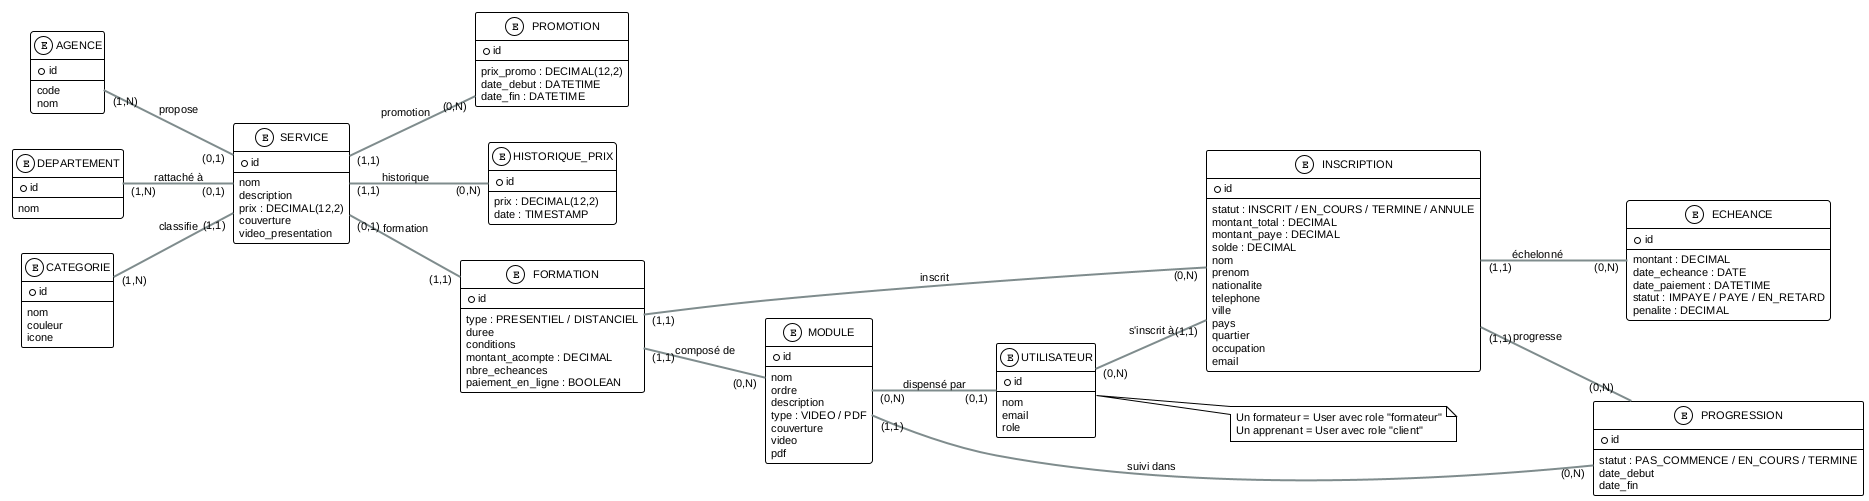
\includegraphics[width=\textwidth]{MCD_Phase2_Coeur_Metier.png}
\end{center}


% ===================================================================
\section{Le MLD expliqué pas à pas}
% ===================================================================

Le MLD (Modèle Logique de Données), c'est le MCD \textbf{transformé en vraies tables} prêtes à être construites dans la base de données (PostgreSQL).

Chaque entité du MCD devient une \textbf{table}. Chaque propriété devient une \textbf{colonne}. Chaque relation devient une \textbf{clé étrangère} (un champ qui pointe vers une autre table).

\subsection{Comment lire une table dans le MLD ?}

\noindent\fcolorbox{secondary}{lightgray!15}{\parbox{\textwidth}{
\texttt{services \{}\\
\hspace*{1cm}\texttt{+ id : uuid PK} \hfill \textcolor{gray}{Clé primaire -- identifiant unique}\\
\hspace*{1cm}\texttt{--}\\
\hspace*{1cm}\texttt{\# agency\_id : uuid FK NULL} \hfill \textcolor{gray}{Clé étrangère vers \texttt{agencies} (optionnelle)}\\
\hspace*{1cm}\texttt{name : varchar(255) NOT NULL} \hfill \textcolor{gray}{Champ obligatoire : nom du service}\\
\hspace*{1cm}\texttt{price : decimal(12,2) NOT NULL} \hfill \textcolor{gray}{Prix (obligatoire)}\\
\hspace*{1cm}\texttt{description : text NULL} \hfill \textcolor{gray}{Description (optionnelle)}\\
\hspace*{1cm}\texttt{created\_at : timestamp NOT NULL} \hfill \textcolor{gray}{Date de création (automatique)}\\
\hspace*{1cm}\texttt{deleted\_at : timestamp NULL} \hfill \textcolor{gray}{Pour la corbeille (soft delete)}\\
\texttt{\}}
}}

\vspace{12pt}

\noindent\begin{tabularx}{\textwidth}{l l X}
    \toprule
    \textbf{Symbole} & \textbf{Nom} & \textbf{Signification} \\
    \midrule
    \texttt{+} & Clé primaire (PK) & Identifiant unique de chaque ligne \\
    \texttt{\#} & Clé étrangère (FK) & Lien vers une autre table \\
    \texttt{NOT NULL} & Obligatoire & On ne peut pas laisser vide \\
    \texttt{NULL} & Optionnel & On peut laisser vide \\
    \texttt{DEFAULT} & Valeur par défaut & Si on ne précise rien, cette valeur est utilisée \\
    \texttt{UNIQUE} & Unique & Pas deux fois la même valeur \\
    \bottomrule
\end{tabularx}

\subsection{Les types de données}

\noindent\begin{tabularx}{\textwidth}{l X}
    \toprule
    \textbf{Type} & \textbf{Ça stocke quoi ?} \\
    \midrule
    \texttt{uuid} & Un identifiant unique universel (ex: \texttt{550e8400-e29b-41d4-a716-446655440000}) \\
    \texttt{varchar(255)} & Un texte court (nom, email, téléphone) \\
    \texttt{text} & Un texte long (description, conditions) \\
    \texttt{decimal(12,2)} & Un nombre avec virgule (prix : 12 chiffres dont 2 après la virgule) \\
    \texttt{integer} & Un nombre entier (durée en jours) \\
    \texttt{boolean} & Vrai ou Faux (oui/non) \\
    \texttt{timestamp} & Une date avec l'heure (ex: \texttt{2026-07-30 14:30:00}) \\
    \texttt{date} & Une date sans l'heure (ex: \texttt{2026-07-30}) \\
    \texttt{bigint} & Un très grand nombre entier (taille en octets) \\
    \bottomrule
\end{tabularx}

% ===================================================================
\section{Les tables du MLD une par une}
% ===================================================================

\subsection{Table \texttt{services}}

\noindent\fcolorbox{secondary}{lightgray!15}{\parbox{\textwidth}{\small
\texttt{services} -- Stocke tous les services et activités proposés par PEKEGNO.\\[4pt]
\noindent\begin{tabularx}{\textwidth}{l l X}
    \textbf{Colonne} & \textbf{Type} & \textbf{Explication} \\
    \midrule
    id & uuid PK & Identifiant unique du service \\
    agency\_id & uuid FK NULL & Agence qui propose ce service (ou rien) \\
    department\_id & uuid FK NULL & Département qui propose ce service (ou rien) \\
    category\_id & uuid FK NOT NULL & Catégorie du service (obligatoire) \\
    name & varchar(255) & Nom du service \\
    description & text & Description détaillée \\
    price & decimal(12,2) & Prix du service \\
    coverage & varchar(50) & Zone de couverture (national, régional, etc.) \\
    presentation\_video & varchar(255) & URL de la vidéo de présentation \\
\end{tabularx}
}}

\subsection{Table \texttt{promotions}}

\noindent\fcolorbox{secondary}{lightgray!15}{\parbox{\textwidth}{\small
\texttt{promotions} -- Les réductions temporaires sur les services.\\[4pt]
\noindent\begin{tabularx}{\textwidth}{l l X}
    \textbf{Colonne} & \textbf{Type} & \textbf{Explication} \\
    \midrule
    id & uuid PK & Identifiant unique \\
    service\_id & uuid FK NOT NULL & Le service concerné par la promo \\
    promotional\_price & decimal(12,2) & Le prix en promo \\
    start\_date & timestamp & Début de la promotion \\
    end\_date & timestamp & Fin de la promotion \\
\end{tabularx}
}}

\subsection{Table \texttt{price\_history}}

\noindent\fcolorbox{secondary}{lightgray!15}{\parbox{\textwidth}{\small
\texttt{price\_history} -- L'historique des changements de prix.\\[4pt]
\noindent\begin{tabularx}{\textwidth}{l l X}
    \textbf{Colonne} & \textbf{Type} & \textbf{Explication} \\
    \midrule
    id & uuid PK & Identifiant unique \\
    service\_id & uuid FK NOT NULL & Le service concerné \\
    price & decimal(12,2) & Le nouveau prix \\
    changed\_by & uuid FK NOT NULL & Qui a fait le changement (utilisateur) \\
    reason & varchar(255) & Pourquoi le prix a changé \\
\end{tabularx}
}}

\subsection{Table \texttt{trainings}}

\noindent\fcolorbox{secondary}{lightgray!15}{\parbox{\textwidth}{\small
\texttt{trainings} -- Les informations spécifiques aux formations.\\[4pt]
\noindent\begin{tabularx}{\textwidth}{l l X}
    \textbf{Colonne} & \textbf{Type} & \textbf{Explication} \\
    \midrule
    id & uuid PK & Identifiant unique \\
    service\_id & uuid FK UNIQUE & Le service associé (unique : 1 formation = 1 service) \\
    type & varchar(20) & \texttt{presentiel} ou \texttt{distanciel} \\
    duration\_days & integer & Durée en jours \\
    conditions & text & Conditions d'accès (prérequis, etc.) \\
    deposit\_amount & decimal(12,2) & Montant de l'acompte (pour présentiel) \\
    installment\_count & integer & Nombre d'échéances (pour présentiel) \\
    has\_online\_payment & boolean & Accepte-t-il le paiement en ligne ? \\
\end{tabularx}
}}

\subsection{Table \texttt{training\_modules}}

\noindent\fcolorbox{secondary}{lightgray!15}{\parbox{\textwidth}{\small
\texttt{training\_modules} -- Les leçons qui composent une formation.\\[4pt]
\noindent\begin{tabularx}{\textwidth}{l l X}
    \textbf{Colonne} & \textbf{Type} & \textbf{Explication} \\
    \midrule
    id & uuid PK & Identifiant unique \\
    training\_id & uuid FK NOT NULL & La formation à qui appartient ce module \\
    trainer\_id & uuid FK NULL & Le formateur (utilisateur) qui enseigne ce module \\
    name & varchar(255) & Nom du module \\
    type & varchar(20) & \texttt{video} ou \texttt{pdf} \\
    sort\_order & integer & Ordre d'affichage (Module 1, Module 2\ldots) \\
    coverage & varchar(50) & Contenu/matière couverte \\
    video\_url & varchar(500) & Lien vers la vidéo (si type = video) \\
    pdf\_url & varchar(500) & Lien vers le PDF (si type = pdf) \\
\end{tabularx}
}}

\subsection{Table \texttt{training\_enrollments}}

\noindent\fcolorbox{secondary}{lightgray!15}{\parbox{\textwidth}{\small
\texttt{training\_enrollments} -- Les inscriptions aux formations.\\[4pt]
\noindent\begin{tabularx}{\textwidth}{l l X}
    \textbf{Colonne} & \textbf{Type} & \textbf{Explication} \\
    \midrule
    id & uuid PK & Identifiant unique \\
    training\_id & uuid FK NOT NULL & La formation concernée \\
    user\_id & uuid FK NULL & L'utilisateur inscrit (NULL si son compte n'est pas encore créé) \\
    status & varchar(20) & \texttt{enrolled}, \texttt{in\_progress}, \texttt{completed}, \texttt{cancelled} \\
    total\_amount & decimal(12,2) & Montant total de la formation \\
    paid\_amount & decimal(12,2) & Montant déjà payé \\
    balance & decimal(12,2) & Reste à payer \\
    first\_name \ldots email & varchar(150)\ldots & Informations du formulaire d'inscription \\
    enrolled\_at & timestamp & Date d'inscription \\
    completed\_at & timestamp & Date de fin (si terminé) \\
\end{tabularx}
}}

\subsection{Table \texttt{training\_installments}}

\noindent\fcolorbox{secondary}{lightgray!15}{\parbox{\textwidth}{\small
\texttt{training\_installments} -- Les échéances de paiement.\\[4pt]
\noindent\begin{tabularx}{\textwidth}{l l X}
    \textbf{Colonne} & \textbf{Type} & \textbf{Explication} \\
    \midrule
    id & uuid PK & Identifiant unique \\
    enrollment\_id & uuid FK NOT NULL & L'inscription concernée \\
    amount & decimal(12,2) & Montant à payer pour cette échéance \\
    due\_date & date & Date limite de paiement \\
    paid\_at & timestamp & Quand a-t-elle été payée ? (NULL si pas encore) \\
    status & varchar(20) & \texttt{unpaid}, \texttt{paid}, \texttt{overdue} \\
    penalty\_amount & decimal(12,2) & Pénalité si en retard \\
\end{tabularx}
}}

\subsection{Table \texttt{training\_module\_progress}}

\noindent\fcolorbox{secondary}{lightgray!15}{\parbox{\textwidth}{\small
\texttt{training\_module\_progress} -- La progression de l'apprenant dans chaque module.\\[4pt]
\noindent\begin{tabularx}{\textwidth}{l l X}
    \textbf{Colonne} & \textbf{Type} & \textbf{Explication} \\
    \midrule
    id & uuid PK & Identifiant unique \\
    enrollment\_id & uuid FK NOT NULL & L'inscription concernée \\
    module\_id & uuid FK NOT NULL & Le module concerné \\
    status & varchar(20) & \texttt{not\_started}, \texttt{in\_progress}, \texttt{completed} \\
    started\_at & timestamp & Quand l'apprenant a commencé \\
    completed\_at & timestamp & Quand l'apprenant a terminé \\
\end{tabularx}
}}

% ===================================================================
\section{Le schéma MLD complet}
% ===================================================================

\begin{center}
    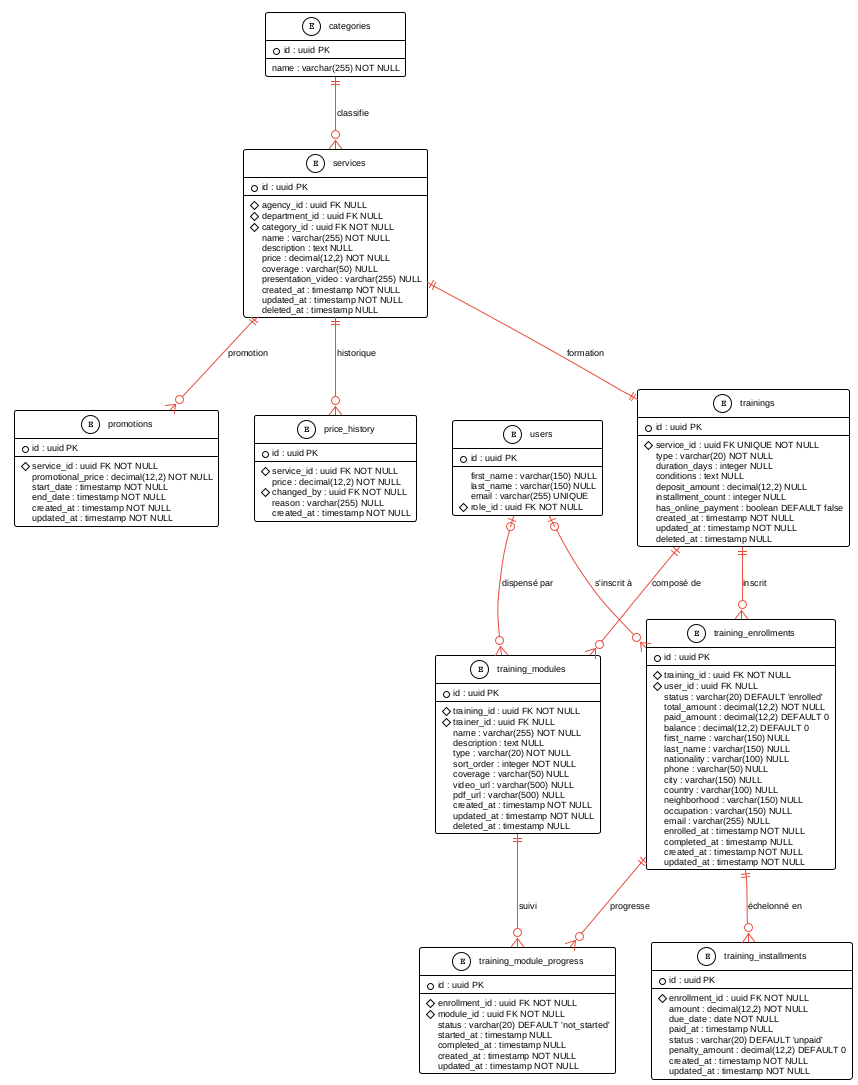
\includegraphics[width=\textwidth]{MLD_Phase2_Coeur_Metier.png}
\end{center}

% ===================================================================
\section{Les relations dans le MLD}
% ===================================================================

\noindent\begin{tabularx}{\textwidth}{l l X}
    \toprule
    \textbf{Table 1} & \textbf{Table 2} & \textbf{Comment ça marche ?} \\
    \midrule
    categories & services & \texttt{services.category\_id} pointe vers \texttt{categories.id}. Chaque service a une catégorie. \\
    services & promotions & \texttt{promotions.service\_id} pointe vers \texttt{services.id}. Chaque promo concerne un service. \\
    services & price\_history & \texttt{price\_history.service\_id} pointe vers \texttt{services.id}. Historique des prix. \\
    services & trainings & \texttt{trainings.service\_id} pointe vers \texttt{services.id}. Un service = une formation (1-1). \\
    trainings & training\_modules & \texttt{training\_modules.training\_id} pointe vers \texttt{trainings.id}. Une formation a plusieurs modules. \\
    users & training\_modules & \texttt{training\_modules.trainer\_id} pointe vers \texttt{users.id}. Un formateur enseigne des modules. \\
    trainings & training\_enrollments & \texttt{training\_enrollments.training\_id} pointe vers \texttt{trainings.id}. Inscriptions à une formation. \\
    users & training\_enrollments & \texttt{training\_enrollments.user\_id} pointe vers \texttt{users.id}. Un apprenant s'inscrit. \\
    training\_enrollments & training\_installments & \texttt{training\_installments.enrollment\_id} pointe vers \texttt{training\_enrollments.id}. Échéances. \\
    training\_enrollments & training\_module\_progress & \texttt{training\_module\_progress.enrollment\_id} pointe vers \texttt{training\_enrollments.id}. Progression. \\
    training\_modules & training\_module\_progress & \texttt{training\_module\_progress.module\_id} pointe vers \texttt{training\_modules.id}. Suivi par module. \\
    \bottomrule
\end{tabularx}

% ===================================================================
\section{Exemple complet : le parcours d'un apprenant}
% ===================================================================

Prenons un exemple du début à la fin pour voir comment toutes les tables travaillent ensemble.

\begin{exemplebox}
\textbf{Histoire :} Koffi veut suivre la formation \textit{« Excel »} proposée par l'agence de Lomé.
\end{exemplebox}

\subsection*{Étape 1 : On crée le service}

\begin{tabularx}{\textwidth}{l X}
    \textbf{Table} & \textbf{Nouvelle ligne} \\
    \midrule
    \texttt{services} & nom = « Formation Excel », price = 50 000 FCFA, \\
    & category = « Informatique », agency = « Agence Lomé » \\
\end{tabularx}

\subsection*{Étape 2 : On crée la formation}

\begin{tabularx}{\textwidth}{l X}
    \textbf{Table} & \textbf{Nouvelle ligne} \\
    \midrule
    \texttt{trainings} & service = « Formation Excel », type = présentiel, \\
    & duration\_days = 5, deposit\_amount = 15 000, \\
    & installment\_count = 2 \\
\end{tabularx}

\subsection*{Étape 3 : On crée les modules}

\begin{tabularx}{\textwidth}{l X}
    \textbf{Table} & \textbf{Nouvelles lignes} \\
    \midrule
    \texttt{training\_modules} & Module 1 : « Les bases », type = video, formateur = Amara \\
    & Module 2 : « Formules », type = video, formateur = Amara \\
    & Module 3 : « Exercices », type = pdf, formateur = Amara \\
\end{tabularx}

\subsection*{Étape 4 : Promotion de la formation}

\begin{tabularx}{\textwidth}{l X}
    \textbf{Table} & \textbf{Nouvelle ligne} \\
    \midrule
    \texttt{promotions} & service = « Formation Excel », prix\_promo = 35 000 FCFA, \\
    & du 1er au 15 août \\
\end{tabularx}

\subsection*{Étape 5 : Koffi paie et s'inscrit}

\begin{tabularx}{\textwidth}{l X}
    \textbf{Table} & \textbf{Nouvelle ligne} \\
    \midrule
    \texttt{training\_enrollments} & training = « Formation Excel », \\
    & user = Koffi (après création de son compte), \\
    & total\_amount = 50 000, paid\_amount = 0, balance = 50 000 \\
\end{tabularx}

\subsection*{Étape 6 : Création des échéances}

\begin{tabularx}{\textwidth}{l X}
    \textbf{Table} & \textbf{Nouvelles lignes} \\
    \midrule
    \texttt{training\_installments} & Échéance 1 : 25 000 FCFA, due le 15/08 \\
    & Échéance 2 : 25 000 FCFA, due le 15/09 \\
\end{tabularx}

\subsection*{Étape 7 : Koffi suit les modules}

\begin{tabularx}{\textwidth}{l X}
    \textbf{Table} & \textbf{Nouvelles lignes} \\
    \midrule
    \texttt{training\_module\_progress} & Module 1 : terminé le 05/08 \\
    & Module 2 : en cours \\
    & Module 3 : pas commencé \\
\end{tabularx}

% ===================================================================
\section{Résumé visuel : qui est qui ?}
% ===================================================================

\noindent\begin{tabularx}{\textwidth}{l l X}
    \toprule
    \textbf{Entité MCD} & \textbf{Table MLD} & \textbf{Dans la vraie vie} \\
    \midrule
    SERVICE & \texttt{services} & Ce que PEKEGNO vend \\
    PROMOTION & \texttt{promotions} & Une réduction temporaire \\
    HISTORIQUE\_PRIX & \texttt{price\_history} & La mémoire des anciens prix \\
    FORMATION & \texttt{trainings} & Une formation (présentiel ou distanciel) \\
    MODULE & \texttt{training\_modules} & Une leçon dans une formation \\
    INSCRIPTION & \texttt{training\_enrollments} & Un apprenant inscrit à une formation \\
    ECHEANCE & \texttt{training\_installments} & Un paiement à faire \\
    PROGRESSION & \texttt{training\_module\_progress} & L'avancement d'un apprenant \\
    \bottomrule
\end{tabularx}

\vspace{12pt}

\begin{resume}
    \textbf{À retenir :}
    \begin{itemize}
        \item Le \textbf{MCD} = le plan conceptuel (quoi ?)
        \item Le \textbf{MLD} = le plan technique (comment ?)
        \item Les \textbf{cardinalités} disent combien de fois les choses sont liées
        \item Les \textbf{clés étrangères (FK)} sont les ponts entre les tables
    \end{itemize}
\end{resume}

\end{document}
